\documentclass[11pt,a4paper]{article}

\usepackage[T1]{fontenc}
\usepackage[utf8]{inputenc}
\usepackage{mathpazo}
\usepackage[margin=2.5cm,top=2.3cm,bottom=2.3cm]{geometry}
\usepackage{amsmath,amssymb}
\usepackage{xcolor}
\usepackage{titlesec}
\usepackage{enumitem}
\usepackage{booktabs}
\usepackage{tabularx}
\usepackage[most]{tcolorbox}
\usepackage{microtype}
\usepackage{needspace}
\usepackage{fancyhdr}
\usepackage{tikz}
\usetikzlibrary{arrows.meta,positioning,calc}
\usepackage[hidelinks]{hyperref}

\definecolor{ifteal}{HTML}{0E5250}
\definecolor{ifclay}{HTML}{B4573C}
\definecolor{ifgrey}{HTML}{5B6770}
\definecolor{ifslate}{HTML}{40607D}
\definecolor{ifrule}{HTML}{D8D2C6}
\definecolor{ifpale}{HTML}{EAF2F1}

\titleformat{\section}{\color{ifteal}\normalfont\Large\bfseries}{\thesection.}{0.5em}{}
\titleformat{\subsection}{\color{ifteal}\normalfont\large\bfseries}{\thesubsection}{0.6em}{}
\titleformat{\subsubsection}{\color{ifclay}\normalfont\normalsize\bfseries}{}{0em}{}
\titlespacing*{\section}{0pt}{18pt}{7pt}
\titlespacing*{\subsection}{0pt}{13pt}{4pt}
\titlespacing*{\subsubsection}{0pt}{10pt}{3pt}

\setlist[itemize]{leftmargin=1.3em,itemsep=2pt,topsep=3pt}
\setlength{\parindent}{0pt}
\setlength{\parskip}{5pt}

\pagestyle{fancy}\fancyhf{}
\renewcommand{\headrulewidth}{0pt}
\fancyfoot[C]{\color{ifgrey}\small\thepage}

\newcommand{\where}[1]{{\color{ifgrey}\small #1\par}}
\newcommand{\step}[2]{\par\nobreak\vspace{2pt}%
  \hangindent=2.0em\hspace*{1.2em}\textcolor{ifteal}{\textbf{#1}}\hspace{0.45em}#2\par}
\newtcolorbox{keybox}{enhanced,breakable,colback=white,colframe=white,
  boxrule=0pt,borderline west={1.6pt}{0pt}{ifclay},
  left=10pt,right=2pt,top=4pt,bottom=4pt,before skip=7pt,after skip=9pt}
\newtcolorbox{probbox}{enhanced,breakable,colback=ifpale,colframe=ifteal,
  boxrule=0.6pt,arc=2pt,left=10pt,right=10pt,top=7pt,bottom=7pt,
  before skip=9pt,after skip=9pt}
\newcommand{\keylab}[1]{\textcolor{ifclay}{\textbf{#1}}}

\begin{document}

\begin{center}
{\color{ifteal}\Huge\bfseries Financial Regulation}\\[5pt]
{\color{ifgrey}\large International Finance --- KEDGE Business School}\\[3pt]
{\color{ifgrey}\itshape Chapter 4 --- the session, written out}
\end{center}
\vspace{5pt}
{\color{ifrule}\hrule height 0.8pt}
\vspace{7pt}

This covers the last chapter of the course in full, including both problems with
their solutions. Read it as you would attend the session: the order is the order
of the slides, and the argument builds. It should take about an hour.

The chapter has one idea running through it, so hold on to it from the start:
\emph{a financial crisis is an information event, and every regulation designed
to prevent one creates a new incentive problem of its own.} Everything below is
an instance of that sentence.

% =========================================================== 1
\section{What a financial crisis is}

A functioning financial system is critical to a robust economy. The basis for
understanding what goes wrong is \textbf{agency theory} --- the study of moral
hazard and adverse selection, which you met in the previous chapter.

Asymmetric information creates barriers between savers and firms with productive
investment opportunities. A saver who cannot tell a good borrower from a bad one
will not lend, or will not lend cheaply. From that follows the definition the
whole chapter uses:

\begin{keybox}
\keylab{Definition.} A financial crisis occurs when information flows in
financial markets experience a particularly large disruption. Financial markets
may then stop functioning completely.
\end{keybox}

Notice what this definition is \emph{not}. It is not about prices falling, and
it is not a synonym for recession. That matters, because it tells you what a
remedy has to do. If the problem were prices, the cure would be to support
prices. Because the problem is information, the cure has to restore the ability
to tell who is solvent --- which is the logic behind every regulation in the
second half of this chapter.

Crises usually proceed in two or three stages.

\subsection*{Stage one --- initiation}

A crisis can begin in any of three ways.

\subsubsection*{Mismanaged financial liberalisation or innovation}
Restrictions are lifted, or new types of loan or financial product are
introduced. This can lead to a \textbf{credit boom} in which risk management is
lacking. Government safety nets make it worse, because depositors who are
insured have no reason to care how much risk their bank is taking. Loan losses
then accrue, asset values fall, and capital falls with them. Institutions cut
back lending --- \textbf{deleveraging} --- and their own funding falls too.

And then the step that matters most: as institutions cut back on lending,
\emph{nobody is left to evaluate firms}. The financial system loses its primary
institution for addressing adverse selection and moral hazard, so spending
contracts as loans become scarce. A sound firm cannot borrow --- not because it
is unsound, but because the machinery for proving soundness has stopped.

\subsubsection*{An asset-price boom and bust}
A pricing bubble starts, where asset values exceed their fundamental values.
When it bursts and prices fall, corporate net worth falls as well, and moral
hazard increases because firms have little left to lose. Financial institutions
also see their assets fall, leading again to deleveraging.

\subsubsection*{An increase in uncertainty}
Periods of high uncertainty can lead to crises: a stock market crash, or the
failure of a major financial institution. In 1857 it was the Ohio Life Insurance
\& Trust Company; in 2008, AIG, Bear Stearns and Lehman Brothers. With
information hard to come by, moral hazard and adverse selection problems
increase, reducing lending and economic activity.

\subsection*{Stage two --- banking crisis}

Deteriorating balance sheets lead financial institutions into insolvency. If
severe enough, this produces a \textbf{bank panic}. Panics occur when depositors
are unsure \emph{which} banks are insolvent, causing all depositors to withdraw
all funds immediately.

That word \emph{which} is the whole mechanism. A panic hits sound banks as well
as unsound ones, because the depositor cannot tell them apart. It is adverse
selection, in a queue outside a branch.

As cash balances fall, institutions must sell assets quickly, further
deteriorating their balance sheets --- and driving down the price of the same
assets held by everyone else. A bank acting prudently makes its neighbour
insolvent. Adverse selection and moral hazard become severe, and it takes years
for a full recovery.

\subsection*{Stage three --- debt deflation}

If the crisis also leads to a sharp decline in the price level, \textbf{debt
deflation} can occur: asset prices fall, but debt levels do not adjust,
increasing debt burdens.

The arithmetic is worth doing. You owe 100, and the price level falls by 25\%.
You have not borrowed another penny, but what you owe has risen by about a third
in real terms. This leads to a further increase in adverse selection and moral
hazard, decreased lending, and economic activity that remains depressed for a
long time.

Stage three requires a fall in the general \emph{price level}, not merely in
asset prices, which is why it does not always happen.

\subsection*{The sequence, in one picture}

\begin{center}
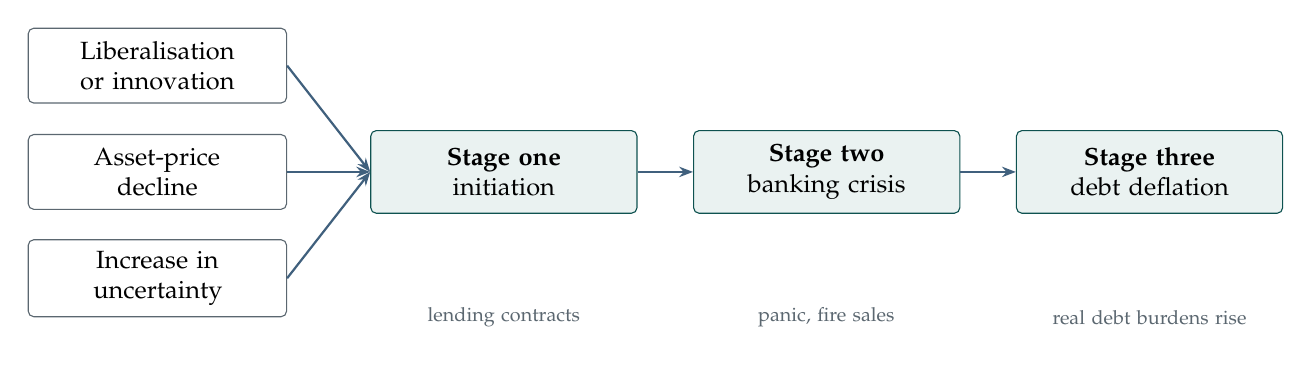
\begin{tikzpicture}[
  font=\small,
  trig/.style={draw=ifgrey,rounded corners=2pt,align=center,inner sep=4pt,
               text width=3.0cm,minimum height=0.95cm},
  stg/.style={draw=ifteal,fill=ifpale,rounded corners=2pt,align=center,
              inner sep=4pt,text width=3.1cm,minimum height=1.05cm},
  ar/.style={-{Stealth[length=5pt]},draw=ifslate,thick}
]
\node[trig] (t1) at (0,2.1) {Liberalisation\\or innovation};
\node[trig] (t2) at (0,0.75) {Asset-price\\decline};
\node[trig] (t3) at (0,-0.6) {Increase in\\uncertainty};
\node[stg] (s1) at (4.4,0.75) {\textbf{Stage one}\\initiation};
\node[stg] (s2) at (8.5,0.75) {\textbf{Stage two}\\banking crisis};
\node[stg] (s3) at (12.6,0.75) {\textbf{Stage three}\\debt deflation};
\foreach \t in {t1,t2,t3} \draw[ar] (\t.east) -- (s1.west);
\draw[ar] (s1) -- (s2);
\draw[ar] (s2) -- (s3);
\node[align=center,text=ifgrey,font=\scriptsize,text width=3.1cm] at (4.4,-1.1)
  {lending contracts};
\node[align=center,text=ifgrey,font=\scriptsize,text width=3.1cm] at (8.5,-1.1)
  {panic, fire sales};
\node[align=center,text=ifgrey,font=\scriptsize,text width=3.1cm] at (12.6,-1.1)
  {real debt burdens rise};
\end{tikzpicture}
\end{center}

At every stage the same thing happens: adverse selection and moral hazard
worsen, and lending contracts. One mechanism, three stages.

% =========================================================== 2
\section{The Great Depression}

In 1928 and 1929, stock prices doubled in the United States. The Fed tried to
curb this period of excessive speculation with a tight monetary policy, but this
led to a market collapse of more than 20\% in October 1929, and a further 20\%
by the end of that year. The decline continued for several years.

What might have been a normal recession turned into something far worse when
severe droughts in 1930 in the Midwest led to a sharp decline in agricultural
production. Between 1930 and 1933, \textbf{one-third of US banks} went out of
business as agricultural shocks produced bank failures. For more than two years
the Fed sat idly by through one bank panic after another.

Adverse selection and moral hazard in credit markets became severe, and firms
with productive uses of funds were unable to get financing. Credit spreads ---
the extra yield demanded of a risky borrower over a safe one --- increased from
\textbf{2\% to nearly 8\%} at the height of the Depression in 1932.

That number is the definition of a crisis, measured. The spread did not widen
because firms became four times worse. It widened because nobody could tell
which firms were which.

\subsubsection*{The consequences}
\begin{itemize}
\item Deflation of \textbf{25\%} in the price level --- stage three, in the data.
\item Unemployment around \textbf{25\%}.
\item The worst financial crisis ever experienced in the United States.
\item Bank panics spread from the US to the rest of the world, and the US
contraction decreased demand for foreign goods.
\item The worldwide depression caused great hardship, and the resulting
discontent led to the rise of fascism and the Second World War.
\end{itemize}

% =========================================================== 3
\section{The Global Financial Crisis}

\subsection*{Three central factors}

\textbf{Financial innovation in mortgage markets.} Less-than-creditworthy
borrowers found the ability to purchase homes through \emph{subprime lending}, a
practice almost nonexistent until the 2000s. Financial engineering then
developed new products to enhance and distribute the risk from that lending.

\textbf{Agency problems.} Mortgage originators did not hold the mortgage; they
sold the note in the secondary market. They earned fees from the \emph{volume}
of loans, not their quality. In the extreme, unqualified borrowers bought houses
they could not afford through creative mortgage products or outright fraud, such
as inflated income.

Follow the chain and the problem becomes obvious: a borrower, an originator, a
bank that buys the note, a special purpose vehicle, a rating agency, an
investor. Ask who loses money if the borrower cannot pay. Only the investor at
the end, and not quickly. Everyone upstream has been paid and has moved on. The
one person close enough to the borrower to verify anything has no stake in
whether the loan is repaid.

\textbf{Asymmetric information in the credit rating process.} Agencies consulted
with firms on structuring products to achieve the highest rating, which is a
clear conflict of interest. The rating system was not designed for the complex
nature of structured debt. The result was ratings that meant very little, and
that investors had relied on to assess the quality of their investments.

\subsection*{Collateralised debt obligations}

A \textbf{special purpose vehicle} (SPV) is created to buy assets, create
securities from those assets, and sell those securities to investors. In a CDO,
the securities --- called \textbf{tranches} --- are created based on default
priorities. The first defaults go to the lowest-rated tranches; the highest
tranches suffer only if most of the assets default.

\begin{center}
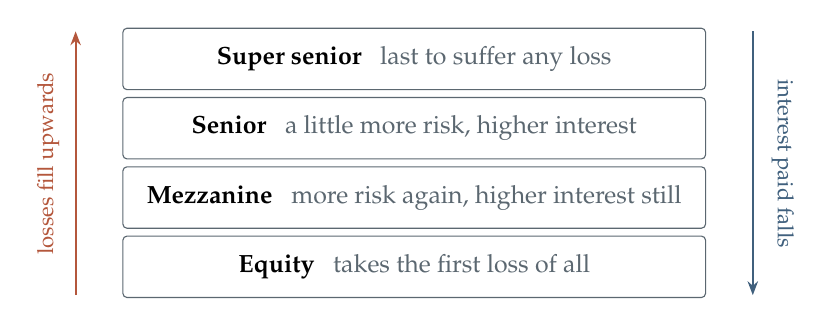
\begin{tikzpicture}[font=\small,
  tr/.style={draw=ifgrey,rounded corners=1.5pt,minimum width=7.4cm,
             minimum height=0.78cm,align=left,inner sep=6pt},
  ar/.style={-{Stealth[length=5pt]},thick}]
\node[tr] (a) at (0,2.40) {\textbf{Super senior} \ \ {\color{ifgrey}last to suffer any loss}};
\node[tr] (b) at (0,1.52) {\textbf{Senior} \ \ {\color{ifgrey}a little more risk, higher interest}};
\node[tr] (c) at (0,0.64) {\textbf{Mezzanine} \ \ {\color{ifgrey}more risk again, higher interest still}};
\node[tr] (d) at (0,-0.24) {\textbf{Equity} \ \ {\color{ifgrey}takes the first loss of all}};
\draw[ar,draw=ifclay] (-4.3,-0.6) -- (-4.3,2.75);
\node[rotate=90,text=ifclay,font=\footnotesize] at (-4.65,1.07) {losses fill upwards};
\draw[ar,draw=ifslate] (4.3,2.75) -- (4.3,-0.6);
\node[rotate=270,text=ifslate,font=\footnotesize] at (4.68,1.07) {interest paid falls};
\end{tikzpicture}
\end{center}

\begin{probbox}
\textbf{Problem 4.1.} What are the risks linked to CDOs?
\end{probbox}

\textbf{Correlation.} The entire structure assumes that defaults are largely
independent of one another. If they are correlated --- and in a national housing
downturn they are --- losses do not stay in the bottom tranches. The senior
tranches fail too. This is the risk the ratings missed, and it is the most
important answer.

\textbf{Opacity and valuation.} Nobody could value these securities quickly.
That is what froze the market in 2007: not that the securities were worthless,
but that nobody could demonstrate they were not.

\textbf{Model and rating risk.} The rating was produced by the agency that had
helped structure the deal, using models not built for the product.

\textbf{Liquidity and funding.} They were held with short-term funding, so a
fall in value forced sales, which forced the value down further.

\begin{keybox}
\keylab{The structural answer.} Tranching does not reduce the total risk of the
pool. It \emph{redistributes} it. The pool is exactly as risky as it was before
it was sliced; what changed is who holds which part --- and how safe the top
part was allowed to look.
\end{keybox}

\subsection*{US residential housing}

Initially the housing boom was lauded by economists and politicians, and it
helped stimulate growth in the subprime market. But underwriting standards fell,
and people were clearly buying houses they could not afford, except through the
ability to sell at a higher price later. That is not lending; it is a bet on an
asset price.

Lending standards also allowed near 100\% financing, so owners had little to
lose by defaulting when the bubble burst. This is moral hazard in debt, with a
number attached: if you put in nothing and the house falls 20\%, walking away
costs you almost nothing. The down payment was never about affordability --- it
was the borrower's stake in not defaulting.

Because of the fall in US housing prices, the number of defaults continued to
plague the banking system. And because every mortgage in those CDOs was secured
on one of these houses, a national fall in house prices is precisely the
correlated event that the tranching assumed away.

\subsection*{Was the Fed to blame?}

Some argue that low interest rates from 2003 to 2006 fuelled the housing bubble
--- rates below what the Taylor rule would have implied. In early 2010 Bernanke
rebutted this, arguing that rates were appropriate and pointing instead to new
mortgage products, relaxed lending standards and capital inflows as more likely
causes. The debate continues.

The useful question is not who is right but what evidence would settle it: you
would want countries with different monetary policies and similar housing booms,
or the reverse.

\subsection*{From mortgages to the system}

As mortgage defaults rose, banks and other institutions saw the value of their
assets fall, complicated by the difficulty of valuing mortgages, CDOs and
default swaps. Banks began deleveraging --- selling assets and restricting
credit --- further depressing the economy. That is stage one, exactly as set out
above.

The \textbf{shadow banking system} also experienced a run: hedge funds,
investment banks and other liquidity providers. These institutions did what
banks do, borrowing short and lending long, without being banks --- and
therefore without deposit insurance or a central bank window as of right. When
the short-term debt markets seized, so did the availability of credit to that
system, leading to further fire sales. It was a bank run in a system with no
deposits and no depositors.

The fall in the stock market and the rise in credit spreads further weakened
firm and household balance sheets, and both consumption and real investment
fell.

\subsection*{The collapse, and what it cost}

Europe was first to raise the alarm. With the downgrade of \$10 billion in
mortgage-related products, short-term money markets froze, and in August 2007 a
French investment house suspended redemption of some of its money market funds.
Banks and firms began to hoard cash. Northern Rock, which relied on short-term
credit markets rather than deposits for funding, was among the first failures;
by most standards Europe experienced a more severe downturn than the US.

Then, in the United States: in March 2008 Bear Stearns failed and was sold to JP
Morgan for 5\% of its value a year earlier. In September 2008, Fannie Mae and
Freddie Mac were put into conservatorship; Lehman Brothers filed for bankruptcy;
Merrill Lynch was sold to Bank of America at fire-sale prices; and AIG
experienced a liquidity crisis.

The crisis caused the worst economic contraction since the Second World War,
peaking in September 2008. Congress passed a bailout package, but the stock
market continued to decline and credit spreads reached over \textbf{500 basis
points}. Real GDP fell and unemployment rose above \textbf{10\%} in 2009. From
March 2009 a bull market began and spreads fell, but the recovery was slow.

\begin{keybox}
\keylab{The comparison that explains the rest of the chapter.} 1932: spreads of
8\%, unemployment of 25\%, deflation of 25\%. 2008: spreads of 5\%, unemployment
of 10\%, no deflation. Why so much less severe? Because this time the central
bank and the government acted, and because deposit insurance meant there was no
queue outside the branch. Sections 4 to 6 below are why 2008 was not 1932.
\end{keybox}

% =========================================================== 4
\section{The European sovereign debt crisis}

Up until 2007, all the countries that had adopted the euro found their interest
rates converging to very low levels. Greek and German borrowing costs were
nearly identical --- which, with hindsight, was an extraordinary thing for a
market to believe.

The currency union had removed exchange rate risk. It had not removed default
risk, and arguably made it worse, because a country inside the union cannot
devalue or print its own way out of a debt problem.

Then several countries were hit at once: lower tax revenue from the economic
contraction, high expenses for financial institution bailouts, and fear of
government default causing rates to surge.

Greece was the first domino. In September 2008 the government projected a 6\%
deficit and 100\% debt-to-GDP. In October, with newly elected officials, the
numbers were shown to be far worse. Fear of default pushed rates on Greek debt
near \textbf{40\%}, and debt-to-GDP rose to \textbf{160\%} by 2012. Greece was
forced to write down its debt --- a partial default --- and civil unrest broke
out as unemployment climbed.

Ireland, Portugal, Spain and Italy followed. Governments were forced to embrace
austerity measures, interest rates climbed to double-digit levels, severe
recessions resulted despite assurances from the ECB, and unemployment rose to
double digits --- \textbf{25\% in Spain}.

Note what kind of crisis this was: the numbers changed when the officials
changed. It was in part an information crisis about the state of the public
accounts, which is the chapter's theme appearing in a different market.

% =========================================================== 5
\section{Asymmetric information and bank capital}

Asymmetric information, moral hazard and adverse selection explain the whole
regulatory environment in banking. This section is the pivot of the chapter: it
shows a remedy working, and then shows what it cost.

\subsection*{Deposit insurance}

Prior to FDIC insurance, bank failures meant depositors lost money, and ``good''
banks needed some way to separate themselves from ``bad'' ones. The inability of
depositors to assess the quality of a bank's assets is what leads to panics ---
and there were major ones in 1819, 1837, 1857, 1873, 1884, 1893, 1907 and
1930--33. Roughly one every fifteen years.

With a government safety net, depositors will not flee the banking system at the
first sign of trouble. Between \textbf{1934 and 1981, fewer than 15 banks failed
each year}. Up to the 1960s only six countries had deposit insurance; by the
1990s the number topped 70.

It is worth being precise about what deposit insurance changed. It did not make
depositors better at judging banks. It removed their \emph{reason to run} ---
and since the run was what turned one bad bank into a system-wide panic, it cut
the link between an individual failure and a general collapse. It makes the
depositor's ignorance harmless rather than trying to cure it.

\subsection*{What deposit insurance costs}

\textbf{Moral hazard.} An insured bank can take greater risk, because the
depositor no longer cares. The depositor was a poor monitor, but they were a
monitor, and the insurance switched them off.

\textbf{Adverse selection.} Those who can take advantage of the insurance are
the ones most likely to find banks attractive. The person who most wants a
licence to lend other people's insured money is precisely the person you would
least like to have one.

\textbf{Too big to fail.} Regulators are reluctant to let the largest banks fail
because of the impact on the entire system. When Continental Illinois failed,
all deposits were insured, and so were the bondholders --- so even creditors
stopped taking an interest in a bank's health. Consolidation has created many
large banks, worsening the problem, and banks now engage in more than banking,
extending the guarantee to activities such as underwriting.

\textbf{The evidence.} Explicit government insurance is associated with less
bank sector stability and more crises, and appears to retard financial
development --- but mainly in countries with ineffective laws, weak regulation
and high corruption. For emerging markets, deposit insurance may be the wrong
medicine.

\begin{keybox}
\keylab{The pattern, stated once.} The cure works by making the depositor
indifferent --- which is exactly the problem. Capital requirements and
supervision exist to replace the monitoring that deposit insurance destroyed.
Every remedy in this chapter has this shape.
\end{keybox}

\subsection*{Restrictions on asset holdings}

Regulations limit the type of assets banks may hold; for instance, banks may not
hold common equity. Even with these regulations in place, the 2007--2009 crisis
still occurred --- the losses came through assets that were permitted and highly
rated. Rules bind the things you thought of.

\subsection*{Capital requirements}

Banks are required to hold a certain level of capital --- book equity ---
depending on the type of assets they hold.

\begin{center}
\renewcommand{\arraystretch}{1.3}
\begin{tabular}{@{}lll@{}}
\toprule
{\color{ifteal}\bfseries Ratio} & {\color{ifteal}\bfseries Definition} & {\color{ifteal}\bfseries Minimum}\\
\midrule
Leverage ratio & capital $\div$ total assets & 4\% \\
Core capital ratio & core capital $\div$ risk-weighted assets & 8.5\% \\
Capital requirement ratio & total capital $\div$ risk-weighted assets & 10.5\% \\
\bottomrule
\end{tabular}
\end{center}

Risk-weighted assets (RWA) means each asset multiplied by a weight reflecting
its risk, including off-balance-sheet activities. Total capital is core capital
plus loan loss reserves.

Why have both kinds of ratio? Because each catches what the other misses. The
leverage ratio is blind to risk, so a bank could satisfy it while holding
nothing but risky assets. The risk-weighted ratios depend on the weights being
right --- and the crisis showed they were not.

Banks engage in \textbf{regulatory arbitrage}: within a given weight category,
every asset counts the same, so they seek the riskiest asset in the bucket. They
are not breaking the rule; they are being paid to find its edges. Every
quantitative rule has this property.

An undercapitalised bank is more likely to fail \emph{and} more likely to engage
in risky activities, which is why the FDIC Improvement Act of 1991 requires the
FDIC to act quickly. ``Well capitalised'' banks are permitted some underwriting
risk; ``undercapitalised'' banks face greater reporting requirements and
oversight.

% ---------------------------------------------------------- problem 4.2
\needspace{18\baselineskip}
\subsection*{Problem 4.2 --- First National Bank}

\begin{probbox}
\textbf{First National Bank} \hfill \textit{\$ millions}\\[4pt]
\begin{tabularx}{\linewidth}{@{}Xr@{\hskip 18pt}Xr@{}}
\textbf{Assets} & & \textbf{Liabilities} & \\
Reserves & 3 & Checkable deposits & 27\\
Treasury securities & 10 & Nontransactions deposits & 65\\
Government agency securities & 7 & Borrowings & 19\\
Municipal bonds & 10 & Loan loss reserves & 2\\
Residential mortgages & 10 & Bank capital & 7\\
Real estate loans & 20 & & \\
Commercial \& industrial loans & 35 & & \\
Fixed assets & 5 & & \\
Letters of credit & 20 & & \\
\end{tabularx}\\[6pt]
\textbf{Risk weights:} 0 for reserves and Treasury securities; 0.2 for
government agency securities; 0.5 for municipal bonds and residential mortgages;
1.0 for real estate loans, C\&I loans, fixed assets and letters of credit.\\[4pt]
Is the leverage ratio respected? Are the core capital and capital requirement
ratios respected?
\end{probbox}

\subsubsection*{Step 1 --- total assets}
$3 + 10 + 7 + 10 + 10 + 20 + 35 + 5 + 20 = \mathbf{120}$. Check the other side:
$27 + 65 + 19 + 2 + 7 = 120$. The balance sheet balances, so nothing has been
misread.

\subsubsection*{Step 2 --- the leverage ratio}
\[ \frac{\text{capital}}{\text{total assets}} = \frac{7}{120} = \mathbf{5.83\%}
   \qquad \text{against a minimum of } 4\% \]
\begin{keybox}
\keylab{Respected.} The bank passes this test comfortably.
\end{keybox}

\subsubsection*{Step 3 --- risk-weighted assets}

\begin{center}
\renewcommand{\arraystretch}{1.15}
\begin{tabular}{@{}lrrr@{}}
\toprule
{\color{ifteal}\bfseries Asset} & {\color{ifteal}\bfseries \$m} & {\color{ifteal}\bfseries Weight} & {\color{ifteal}\bfseries Weighted}\\
\midrule
Reserves & 3 & 0 & 0 \\
Treasury securities & 10 & 0 & 0 \\
Government agency securities & 7 & 0.2 & 1.4 \\
Municipal bonds & 10 & 0.5 & 5.0 \\
Residential mortgages & 10 & 0.5 & 5.0 \\
Real estate loans & 20 & 1.0 & 20.0 \\
Commercial \& industrial loans & 35 & 1.0 & 35.0 \\
Fixed assets & 5 & 1.0 & 5.0 \\
Letters of credit & 20 & 1.0 & 20.0 \\
\midrule
\textbf{Risk-weighted assets} & & & \textbf{91.4}\\
\bottomrule
\end{tabular}
\end{center}

\subsubsection*{Step 4 --- the two risk-weighted ratios}
Core capital is the bank capital, 7:
\[ \frac{7}{91.4} = \mathbf{7.66\%} \qquad \text{against a minimum of } 8.5\% \]
Total capital adds the loan loss reserves, $7 + 2 = 9$:
\[ \frac{9}{91.4} = \mathbf{9.85\%} \qquad \text{against a minimum of } 10.5\% \]
\begin{keybox}
\keylab{Neither is respected.} The bank fails both risk-weighted tests.
\end{keybox}

\subsubsection*{What the problem is testing}

The bank passes the test that ignores risk and fails both that do not. The
reason is the composition of its assets: 80 of its 120 of assets carry a full
risk weight. A bank holding the same capital against Treasury securities would
pass everything.

The shortfalls are small. For the core ratio, $8.5\% \times 91.4 = 7.77$, so it
is about \textbf{0.77} short. For the total ratio, $10.5\% \times 91.4 = 9.60$,
so about \textbf{0.60} short. Small numbers --- and still a breach.

\begin{keybox}
\keylab{Try this yourself.} Move the \$20m of letters of credit into Treasury
securities. RWA falls to 71.4, so the core ratio becomes $7 \div 71.4 = 9.8\%$
and the total ratio $9 \div 71.4 = 12.6\%$. Both now pass, with no new capital
raised --- which is regulatory arbitrage in one line.
\end{keybox}

% =========================================================== 6
\section{Banking regulation}

\subsection*{The Basel Accord, and Basel 3}

In June 1999 the Basel Committee proposed reforms to the original Basel Accord
with three components: linking capital requirements to actual risk for large
international banks; strengthening the supervisory process; and increasing
market discipline mechanisms. Those are the three things a regulator can do ---
set a rule, look at the bank, or make the bank tell everyone else what it is
doing.

Implementation was complex and delayed by years, and only the largest US banks
were ever subject to Basel 2; others followed a simplified standard.

The 2007--2009 crisis revealed three problems with the accord. The capital
required was not enough to weather the crisis. The weights relied on credit
ratings, which were unreliable. And the standards were \textbf{procyclical},
restricting credit exactly when it was most needed. Basel 3, implemented by
2019, addressed the quality of capital, procyclicality, and the credit rating
rules.

\begin{keybox}
\keylab{Procyclicality, explained.} A downturn starts, losses arrive, capital
falls --- and the rule requires the bank to rebuild capital, which means raising
equity in a falling market or shrinking its lending. Every bank does this at the
same time, so credit is withdrawn from the economy precisely when the economy
most needs it. The rule designed to make each bank safe makes the system more
fragile.
\end{keybox}

\subsection*{Supervision and risk management}

Financial supervision is used to reduce the adverse selection problem of
risk-takers: banking attracts them, and you cannot tell them apart from the
outside, so you look. Examinations assign a rating to a bank, used to justify
cease orders for risky activities. There is periodic reporting and frequent
examination, and banks can be declared a ``problem bank'' and examined more
often.

Past examinations focused primarily on the quality of assets. The new trend
focuses on whether the bank may take excessive risk in the near future ---
because asset quality is backward-looking, and by the time assets are visibly
bad it is too late. Four elements are assessed: the quality of board and senior
management oversight; the adequacy of policies limiting risk activity; the
quality of risk measurement and monitoring; and the adequacy of internal
controls to prevent fraud. \textbf{Stress testing} is the formal version of the
same idea --- not what you are worth today, but what you would be worth if
things went badly.

\subsection*{Disclosure, and mark-to-market accounting}

Better information reduces both moral hazard and adverse selection, which is why
disclosure is a regulatory tool at all. Sarbanes-Oxley increased requirements
for accurate accounting statements and put limits on conflicts of interest.

In theory, market prices provide the best basis for estimating the true value of
assets, and hence of capital. But \textbf{mark-to-market} accounting has a major
flaw: the price of an asset during a time of financial distress does not reflect
its fundamental value. If banks must show ``market'' value in their records, a
bank may appear undercapitalised even though the prices are not accurate.

Notice when this criticism was made: in 2007--2009, when asset values were
falling --- not in the early 2000s, when prices were booming and the same
accounting made balance sheets look very good. The argument can be sound and the
people making it not disinterested. Both are true at once, and seeing that is
what separates an analyst from an advocate.

\subsection*{Consumer protection}

Interest rates are standardised as the APR, which helps prevent discrimination.
The deeper point is that standardisation exists so that two offers can be
compared: without a common definition the consumer cannot compare, and if they
cannot compare, competition disciplines nobody. A disclosure rule is a
competition policy.

The crisis revealed a further need. During the housing boom, originators had
little incentive to ensure subprime borrowers could repay. One infamous mortgage
was dubbed the \textbf{NINJA} loan --- no income, no job, no assets.

Ask who, in that transaction, behaved irrationally. Arguably nobody: the
borrower got a house with no money down; the originator got a fee and sold the
note; the buyer of the note held a rated security. Each link behaved sensibly,
and the chain was insane. That is an incentive failure, not a stupidity failure.

In July 2008 the Federal Reserve required mortgages to consider ability to
repay, banned no-doc loans, banned prepayment penalties and required escrow
accounts. A new consumer financial protection agency took responsibility for
most financial products used by a typical consumer.

\subsection*{Competition, and the macroprudential turn}

Branching restrictions reduce competition between banks, and the separation of
banking and securities industries prevented nonbanks from competing --- repealed
in 1999. Less competition can mean higher fees and less innovation, so there is
a genuine trade-off: restricting competition makes banks safer and banking
worse.

\textbf{Micro} regulation focuses on individual banks, and is not enough in a
financial crisis. \textbf{Macro} regulation looks at the banking system as a
whole: damping the leverage cycle that feeds asset bubbles by offering more
lending, and requiring a higher \emph{net stable funding ratio} --- the share of
short-term funding in total funding.

\begin{keybox}
\keylab{The fallacy of composition.} Every bank can be individually safe while
the system is unsafe. You have now seen it twice: the procyclical capital rule
that forces all banks to shrink together, and the fire sale in which every bank
selling a sound asset makes it unsound. That is the entire case for
macroprudential regulation.
\end{keybox}

Bank regulation abroad is similar to that in the US because the problems are
similar, but international banking can readily shift business from one country
to another, requiring coordination between regulators. Basel attempts this, and
these agreements do not solve all international problems --- which is regulatory
arbitrage again, played at the level of countries.

\subsection*{E-finance and electronic banking}

Electronic banking has created new regulatory issues, particularly security and
privacy. An incident in Russia in 1995, where a computer programmer moved
millions from Citibank accounts to personal accounts, illustrates the point. It
creates a need to assess the \emph{technical} skills of banks to handle
transactions securely, and electronic signatures had to be given legal effect.
Privacy laws restrict the sharing of customer information, and this regulation
is likely to keep evolving.

The idea worth keeping: a regulator supervising an electronic bank needs
technical competence, not only financial competence.

% =========================================================== 7
\section{The Dodd-Frank Act, July 2010}

Five categories, and each answers something from earlier in the chapter.

\begin{itemize}
\item \textbf{Consumer protection.} A Consumer Financial Protection Bureau to
examine and enforce regulation of financial products marketed to poor people ---
the answer to the NINJA loan.
\item \textbf{Resolution authority.} Government authority over financial firms
posing a risk to the overall system --- the answer to Lehman, where there was no
orderly way to close a large firm.
\item \textbf{Systemic risk regulation.} A Financial Stability Oversight Council
to monitor markets for asset price bubbles and systemic risk, liquidity
requirements and the liquidation of troubled firms --- the macroprudential turn,
given an institution.
\item \textbf{The Volcker rule.} Banks limited in trading with their own money,
and allowed to own only a small percentage of hedge and private equity funds.
Deposit insurance subsidises a bank's funding, so that funding should not be
used to speculate for the bank's own account.
\item \textbf{Derivatives.} Standardised products traded on exchanges, higher
capital requirements for custom products, some bank dealing operations banned,
and more disclosure --- the answer to AIG, where nobody knew who was exposed.
\end{itemize}

\subsection*{What it leaves open}

\textbf{Too big to fail} is not resolved. Addressing it would mean breaking up
large institutions, either by creating smaller companies out of the whole or by
restricting asset size. Large institutions oppose this because synergies are
eliminated, which may reduce banking efficiency --- an efficiency argument, not
merely a lobbying one. Capital requirements, regulation and supervision are
likely to be strengthened instead.

\textbf{Compensation.} Bonuses are paid out over a number of years and only if
the firm has remained in good health. Such \emph{clawbacks} may encourage
employees to reduce the riskiness of their activities --- the principal-agent
problem with a contractual fix.

\textbf{Government-sponsored enterprises.} The fate of Fannie Mae and Freddie
Mac has not been addressed; several routes exist, each with drawbacks.

\textbf{Credit rating agencies.} Regulation has been strengthened to restrict
conflicts of interest and give incentives for reliable ratings, and more is
likely.

\begin{keybox}
\keylab{The sentence the chapter ends on.} More regulation is needed to prevent
a crisis from ever occurring again --- although there is a substantial danger
that too much, or poorly designed, regulation could hamper the efficiency of the
financial system.
\end{keybox}

There is no setting of the dial that is simply correct. Deposit insurance
stopped the runs and switched off the monitors. Capital rules made banks safer
and made downturns deeper. Mark-to-market told the truth, and told it at the
worst possible moment. An answer to ``should there be more regulation or less''
that does not acknowledge this trade-off is not an answer.

% =========================================================== exam
\section*{\color{ifteal}What you should be able to do}

\begin{itemize}
\item \textbf{State the definition of a financial crisis} and say why it is
about information rather than about prices.
\item \textbf{Set out the three triggers and the three stages}, and say what
worsens at every stage --- adverse selection and moral hazard, so lending
contracts.
\item \textbf{Explain one crisis in terms of that mechanism.} Any of the three
will do; you do not need to memorise all three narratives.
\item \textbf{Explain the risks in a CDO}, and in particular why correlated
defaults break the tranching, and that tranching redistributes risk rather than
reducing it.
\item \textbf{Compute all three capital ratios} from a balance sheet and a set
of risk weights, and interpret the pattern of passes and failures.
\item \textbf{Explain deposit insurance both ways} --- what problem it solves,
and the moral hazard, adverse selection and too-big-to-fail problems it creates.
\item \textbf{Explain procyclicality} and the fallacy of composition behind
macroprudential regulation.
\item \textbf{Give the trade-off} behind any regulation in the chapter, rather
than just naming it.
\end{itemize}

\vspace{8pt}
{\color{ifrule}\hrule height 0.6pt}
\vspace{4pt}
{\color{ifgrey}\small\itshape Slides and course materials:
lauradcontreras.github.io/international-finance-kedge}

\end{document}
